\chapter{Θετικοί και αρνητικοί αριθμοί}
\section{Θετικοί και Αρνητικοί Αριθμοί (Ρητοί αριθμοί) -
H ευθεία των ρητών - Τετμημένη σημείου}
\begin{exercise}
\sel[4]{117} 
Στα ζεύγη αριθμών που ακολουθούν να βρεις ποιοι αριθμοί είναι ομόσημοι και ποιοι είναι ετερόσημοι: (α) 3 και +3, (β) 2 και 5, (γ) –2 και –4, (δ) 7 και +9, (ε) –2 και 1,(στ) 17 και –20, (ζ) –9 και –3,2, (η) –10,5 και 11, (θ) –3 και –100, (ι) +6,7 και +12,3
\end{exercise}

Αργότερα θα μάθεις έναν εύκολο τρόπο για να ελέγξεις αν δύο αριθμοί είναι ομόσημοι οι ετερόσημοι, με όσα έχεις δει μέχρι τώρα μπορείς να το κάνεις ως εξής:
\begin{lstlisting}
    while (True):
        a = float(input('α> '))
        b = float(input('β> '))

        if a > 0:
            if b > 0:
                print("Ομόσημοι")
            else:
                print("Ετερόσημοι")
        else:
            if b < 0:
                print("Ομόσημοι")
            else:
                print("Ετερόσημοι")
\end{lstlisting}
και το αποτέλεσμα θα είναι:
\begin{lstlisting}
α>3
β>+3
Ομόσημοι
α>2
β>5
Ομόσημοι
α>-2
β>-4
Ομόσημοι
α>7
β>+9
Ομόσημοι
α>-2
β>1
Ετερόσημοι
α>17
β>-20
Ετερόσημοι
α> -9
β> -3.2
Ομόσημοι
α> -10.5
β> 11
Ετερόσημοι
α> -3
β> -100
Ομόσημοι
α> 6.7
β> 12.3
Ομόσημοι
\end{lstlisting}

\begin{exercise}
\sel[6]{117} Βρες τη λέξη που σχηματίζεται από τα γράμματα με τετμημένες –6, 10, 9, –9, 5, –5, 0 στο παρακάτω σχήμα. Στη συνέχεια γράψε μ’ αυτό τον τρόπο ένα όνομα που σου αρέσει.
Εικόνα
\end{exercise}
Οι αντιστοιχίσεις μπορούν να αποθηκευτούν σε ένα λεξικό και να βρούμε τη λέξη ως εξής:
\begin{lstlisting}
antistoixiseis = {-11:'Ψ',
-10:'Φ',
-9:'T',
-8:'Ρ',
-7:'Ξ',
-6:'Μ',
-5:'Κ',
-4:'Θ',
-3:'Ζ',
-2:'Δ',
-1:'Β',
0:'Ο',
1:'Α',
2:'Γ',
3:'Ε',
4:'Η',
5:'Ι',
6:'Λ',
7:'Ν',
8:'Π',
9:'Σ',
10:'Υ',
11:'Χ',
12:'Ω'}
tetmimenes = [-6,10,9,-9,5,-5,0]
for i in tetmimenes:
    print(antistoixiseis[i])
\end{lstlisting}

Το αποτέλεσμα θα είναι:
\begin{lstlisting}
Μ
Υ
Σ
T
Ι
Κ
Ο
\end{lstlisting}
Αν αλλάξουμε την εντολή print ως εξής:
\begin{lstlisting}
print(antistoixiseis[i],end='')
\end{lstlisting}
Θα προκύψει:
\begin{lstlisting}
ΜΥΣΤΙΚΟ
\end{lstlisting}
Με το end='' δίνουμε την οδηγία στην Python να μην αλλάζει γραμμή μετά από κάθε print.
H κωδικοποίηση γίνεται με το ίδιο λεξικό αλλά ως εξής:
\begin{lstlisting}
lexi = 'ΜΗΝΥΜΑ'
for l in lexi:
    print(list(antistoixiseis.keys())[
        list(antistoixiseis.values()).index(l)],
          end=',')
\end{lstlisting}
Ο λόγος για τον οποίο είναι τόσο πολύπλοκη η κωδικοποίηση είναι ότι το λεξικό δεν μπορεί να υποστηρίξει και τις δύο κατευθύνσεις πρόσβασης. Ένας εναλλακτικός τρόπος αναπαράστασης των ίδιων δεδομένων θα ήταν ο εξής:
\begin{lstlisting}
grammata = ['Ψ','Φ','T','Ρ','Ξ','Μ','Κ','Θ','Ζ','Δ','Β','Ο','Α','Γ','Ε','Η','Ι','Λ','Ν','Π','Σ','Υ','Χ','Ω']
arithmoi = [-11,-10,-9,-8,-7,-6,-5,-4,-3,-2,-1,0,1,2,3,4,5,6,7,8,9,10,11,12]

tetmimenes = [-6,10,9,-9,5,-5,0]
for i in tetmimenes:
    print(grammata[arithmoi.index(i)],end='')
print()

lexi = 'ΜΗΝΥΜΑ'
for l in lexi:
    print(arithmoi[grammata.index(l)],end=',')
\end{lstlisting}
που δίνει το σωστό αποτέλεσμα:
\begin{lstlisting}
ΜΥΣTΙΚΟ
-6,4,7,10,-6,1,
\end{lstlisting}
\begin{exercise}
\sel[7]{117}
Τα σημεία Α και Β έχουν τετμημένες α και β, αντίστοιχα. Να βρεθεί η τετμημένη του μέσου Μ του τμήματος ΑΒ όταν: (α) α = +5 και β = +8, (β) α = –4 και β = –13.
\end{exercise}
\begin{lstlisting}
>>> (5+8)/2
6.5
>>> (-4+(-13))/2
-8.5
\end{lstlisting}
\section{Απόλυτη τιμή}
Να συμπληρώσεις τον πίνακα που ακολουθεί:
\begin{table}[h]
\begin{tabular}{|c|c|c|c|c|c|c|}
\hline
Αριθμός& -2,73 & +7,66 & -1,05 & 0,+8,07 & -8\\\hline
Aπόσταση του σημείου που αντιστοιχεί από την αρχή του άξονα &&&&&\\\hline
\end{tabular}
\end{table}

Γνωρίζουμε ότι η απόσταση από την αρχή του άξονα είναι η απόλυτη τιμή. Η python μπορεί να υπολογίσει την απόλυτη τιμή με την ειδική εντολή abs, τα τρία πρώτα γράμματα της λέξης absolute.
Οπότε έχουμε:
\begin{lstlisting}
>>> abs(-2.73)
2.74
>>> abs(+7.66)
7.66
>>> abs(-1.05)
1.05
>>> abs(0)
0
>>> abs(+8.07)
8.07
>>> abs(-8)
8
\end{lstlisting}
\begin{exercise}
\sel[3]{121}
ΣΩΣΤΟ ή  ΛΑΘΟΣ
(α) Iσχύει η ανισότητα: $–5,7 < 5,7$. 

(β) Ισχύει η ανισότητα: $–7,6 > –6,7$. 

(γ) Στην ανισότητα $2,3 < x < 4,7$ ο x μπορεί να πάρει 2 ακέραιες τιμές. 

(δ) Υπάρχουν 5 ακριβώς ακέραιοι που αληθεύουν τη σχέση: $–2 \leq x \leq 2$.

(ε) Δύο ακέραιοι με αντίθετο πρόσημο είναι αντίθετοι.
\end{exercise}
(α)
\begin{lstlisting}
>>> -5.7 < 5.7
True
\end{lstlisting}
Σωστό
(β)
\begin{lstlisting}
>>> -7.6 > -6.7
False
\end{lstlisting}
Λάθος
(γ) 
\begin{lstlisting}
for i in range(10):
    if i > 2.3 and i < 4.7:
        print(i)
\end{lstlisting}
το αποτέλεσμα είναι:
\begin{lstlisting}
3
4
\end{lstlisting}
Ο x μπορεί να πάρει 2 ακέραιες τιμές άρα ΣΩΣΤΟ.
(δ)
\begin{lstlisting}
for i in range(-3,3):
    if i >= -2 and i <= 2:
        print(i)
\end{lstlisting}
το αποτέλεσμα είναι:
\begin{lstlisting}
-2
-1
0
1
2
\end{lstlisting}
Υπάρχουν 5 ακριβώς ακέραιοι που αληθεύουν τη σχέση άρα ΣΩΣΤΟ
(ε) Λάθος γιατί υπάρχει η εξαίρεση του μηδενός.

\begin{exercise}
\sel[4]{121} Βρες την απόλυτη τιμή των ρητών: (α) +7,25, (β) –2,5, (γ) +16, (δ) –20,05, (ε) –58.
\end{exercise}
\begin{lstlisting}
>>> abs(+7.25)
7.25
>>> abs(-2.5)
2.5
>>> abs(+16)
16
>>> abs(-20.05)
20.05
>>> abs(-58)
58
\end{lstlisting}
\begin{exercise}
\sel[5]{121}Βρες τους αριθμούς που έχουν ως απόλυτη τιμή: (α) 100, (β) 21,7, (γ) 0, (δ) 7,03, (ε) 5,2.
\end{exercise}
\begin{lstlisting}
def fromabs(x):
    if x == 0:
        return(0)
    else:
        return((x, -x))

>>> fromabs(100)
(100, -100)
>>> fromabs(21.7)
(21.7, -21.7)
>>> fromabs(0)
0
>>> fromabs(7.03)
(7.03, -7.03)
>>> fromabs(5.2)
(5.2, -5.2)
\end{lstlisting}
\begin{exercise}
\sel[6]{121}
Συμπλήρωσε τον πίνακα:
\begin{table}[h]
\begin{tabular}{|c|c|c|c|c|c|c|c|c|}
\hline
Αριθμός      &1&           &         &-19&   &    & & \\\hline
Αντίθετος    & &           &         &   & -8& 12 & & \\\hline
Απόλυτη τιμή & &\multicolumn{2}{c}{2}&   &   &    &\multicolumn{2}{c}{7}\\\hline
\end{tabular}
\end{table}
\end{exercise}
Μπορούμε να χρησιμοποιήσουμε την abs και την fromabs για να βρούμε κάποια στοιχεία του πίνακα ο οποίος διαρμορφώνεται ως εξής:
\begin{table}[h]
\begin{tabular}{|c|c|c|c|c|c|c|c|c|}
\hline
Αριθμός      &1 &   2       &    -2   &-19& 8 & -12& 7&-7\\\hline
Αντίθετος    &-1&  -2       &     2   &19 & -8& 12 &-7& 7\\\hline
Απόλυτη τιμή &1 &\multicolumn{2}{c}{2}& 19& 8 & 12 &\multicolumn{2}{c}{7}\\\hline
\end{tabular}
\end{table}

\begin{exercise}
\sel[7]{121}Toποθέτησε στον άξονα $x'Οx$ τα σημεία με τετμημένες:$–9$, $–5,5$, $+8$, $-3$, $-7,25$, $+1$, $+12$, $+3$, $+9$. 
Ποια από αυτά είναι συμμετρικά ως προς την αρχή του άξονα;
\end{exercise}
\begin{lstlisting}
import matplotlib.pyplot as plt

plt.clf()
points = [(-9,0), (-5.5,0), (8,0), (-3,0), (-7.25,0), (+1,0), (+12,0), (+3,0), (+9,0)]
pointName = ['Α','Β','Γ','Δ','Ε','Ζ','Η','Θ','Ι']
x = [p[0] for p in points]
y = [p[1] for p in points]
plt.grid()
plt.scatter(x,y, s=100 ,marker='o')
for (i,p) in enumerate(points):
    plt.annotate(pointName[i],(p[0],p[1]))

plt.show()
\end{lstlisting}
Που δίνει το αποτέλεσμα:
\begin{figure}[h]
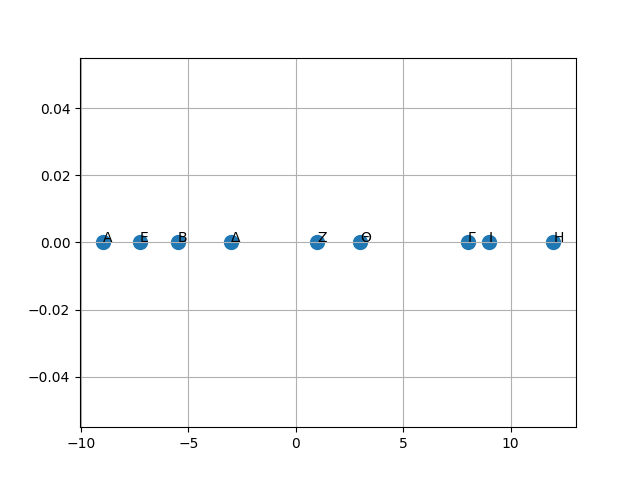
\includegraphics{graph10.png}
\end{figure}
Για να δούμε ποια είναι συμμετρικά θα πρέπει να δούμε ποια ζευγάρια έχουν τις ίδιες απόλυτες τιμές:
\begin{lstlisting}
    l = [-9, -5.5, 8, -3, -7.25, +1, +12, +3, +9]
    for i in l:
        apTimi = abs(i)
        for j in l:
            if apTimi == abs(j) and i != j:
                print(i,j)
\end{lstlisting}
Που δίνει το αποτέλεσμα:
\begin{lstlisting}
-9 9
-3 3
3 -3
9 -9
\end{lstlisting}
\begin{exercise}
\sel[8]{121}
Σχεδίασε τον άξονα $x'Ox$, με κατάλληλη μονάδα για να παραστήσεις τα σημεία με
τετμημένες τους αριθμούς: $–20,5$, $+15$, $–39,75$, $–68,25$, $+70$, $+52,25$,$+43$, $–69$.
\end{exercise}
\begin{lstlisting}
import matplotlib.pyplot as plt

plt.clf()
points = [(-20.5,0), (+15,0), (-39.75,0), (-68.25,0), (+70,0), (+52.25,0), (+43,0), (-69,0)]
pointName = ['Α','Β','Γ','Δ','Ε','Ζ','Η','Θ']
x = [p[0] for p in points]
y = [p[1] for p in points]
plt.grid()
plt.scatter(x,y, s=100 ,marker='o')
for (i,p) in enumerate(points):
    plt.annotate(pointName[i],(p[0],p[1]))

plt.show()
\end{lstlisting}
Που δίνει το αποτέλεσμα:
\begin{figure}[h]
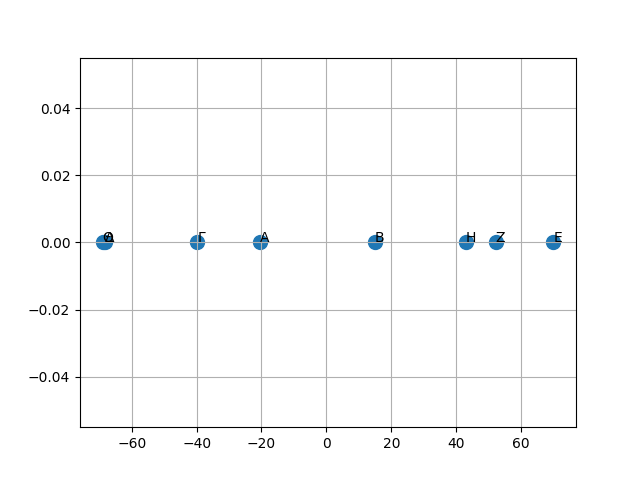
\includegraphics{graph11.png}
\end{figure}
Έτσι βλέπουμε ότι η python επέλεξε μια μονάδα να αντιστοιχεί στο 20 (1:20) και σε αυτή τη κλίμακα είναι αδύνατο να διακρίνουμε τους αριθμούς $-69$ και $-68,25$.
\begin{exercise}
Να συγκρίνεις τους αριθμούς: (α) +41 και +38, (β) 9 και 11, (γ) –3 και –2, (δ) –9 και –16, (ε) 7 και –8, (στ) 0 και –3, (ζ) 0 και +4.
\end{exercise}
\begin{lstlisting}
>>> 41 > 38
True
>>> 9 < 11
True
>>> -3 < -2
True
>>> -9 > -16
True
>>> 7 > -8
True
>>> 0 > -3
True
>>> 4 > 0
True
\end{lstlisting}
\begin{exercise}
\sel[10]{121}
Να συγκρίνεις τους αριθμούς: (α) $11$, $–11$ και $|11|$, (β) $–3$, $+3$ και $|3|$. Τι συμπεραίνεις;
\end{exercise}
\begin{lstlisting}
>>> 11 == abs(11)
True
>>> -11 < abs(11)
True
>>> -3 < abs(3)
True
>>> 3 == abs(3)
True
\end{lstlisting}
\begin{exercise}
\sel[11]{121}
Να γράψεις τους αριθμούς: –2, +7, +15, –3, 0, –4, +5, –8 και –10 σε αύξουσα σειρά.
\end{exercise}
\begin{lstlisting}
>>> print(sorted([-2, +7, +15, -3, 0, -4, +5, -8, -10]))
[-10, -8, -4, -3, -2, 0, 5, 7, 15]
\end{lstlisting}
\begin{exercise}
\sel[12]{121}
Να συμπληρώσεις με το κατάλληλο σύμβολο: <, > ή = τα κενά, ώστε να προκύψουν
αληθείς σχέσεις: (α) $–3 \ldots –8$, (β) $–4 \ldots 10$, (γ) $0 \ldots –1$, (δ) $+3 \ldots 0$, (ε) $–5 \ldots –|–5|$,
(στ) $–5 \ldots –(+5)$, (ζ) $|+7| \ldots |–7|$, (η) $–(–8) \ldots –8$, (θ) $+3 \ldots –(+4)$, (ι) $0 \ldots –|–4|$.
\end{exercise}
\begin{lstlisting}
>>> -3 > -8
True
>>> -4 < 10
True
>>> 0 > -1
True
>>> 3 > 0
True
>>> -5 == -abs(-5)
True
>>> -5 == -(+5)
True
>>> abs(+7) == abs(-7)
True
>>> -(-8) > -8
True
>>> 3 > -(+4)
True
>>> 0 > -abs(-4)
True
\end{lstlisting}

\begin{exercise}
Το x παριστάνει έναν ακέραιο αριθμό. Για ποιες τιμές του x θα ισχύουν οι σχέσεις:
(α) $–13 < x < –8$, (β) $–4 > x > –5$, (γ) $–2 < x < 5$.
\end{exercise}
\begin{lstlisting}
>>> for i in range(-14,-7):
    if i > -13 and i < -8:
        print(i) 
-12
-11
-10
-9
>>> for i in range(-6,0):
    if i < -4 and i > -5:
        print(i) 

>>> for i in range(-3,6):
    if i>-2 and i<5:
        print(i)
-1
0
1
2
3
4
\end{lstlisting}
\section{Πρόσθεση ρητών αριθμών}
\begin{exercise}
\sel[1]{123}
Σε μια πόλη παρατηρήθηκαν οι παρακάτω αυξομειώσεις της θερμοκρασίας:
Αρχικές θερμοκρασίες Αυξομειώσεις θερμοκρασίας

(α) Βράδυ +1°C την επόμενη μέρα αυξήθηκε κατά 4°C

(β) Μεσημέρι –1°C το βράδυ μειώθηκε κατά 2°C

(γ) Βράδυ –2°C την επόμενη μέρα αυξήθηκε κατά 5°C

(δ) Μεσημέρι +5°C το βράδυ μειώθηκε κατά 7°C

(ε) Μεσημέρι –3°C το βράδυ μειώθηκε κατά 3°C
\end{exercise}
\begin{lstlisting}
>>> 1 + 4
5
>>> -1 + (-2)
-3
>>> -2 + 5
3
>>> 5 + (-7)
-2
>>> +3 + (-3)
0
\end{lstlisting}
\begin{exercise}
\sel[2]{124}
Να υπολογιστούν τα παρακάτω αθροίσματα:
(α) $(+5,6) + (+8,7) + (-3,2) + (-6,9) + (+3,2) + (-7,4)$ και
(β) $(-1,8) + (+4,8) + (+9,7) + (-4,8) + (-3,4) + (+1,5)$.
\end{exercise}
\begin{lstlisting}
>>> (+5.6) + (+8.7) + (-3.2) + (-6.9) + (+3.2) + (-7.4)
-2.6645352591003757e-15
\end{lstlisting}
Στην ουσία το αποτέλεσμα είναι 0, αυτός ο αριθμός είναι πολύ μικρός.
\begin{lstlisting}
>>> (-1.8) + (+4.8) + (+9.7) + (-4.8) + (-3.4) + (+1.5)
6.0
\end{lstlisting}

\begin{exercise}
\sel[2]{125}
Υπολόγισε τα αθροίσματα:
(α) (+4,05) + (+6,15), 

(β) (+5,03) + (+4,07), 

(γ) (+2,7) + (+97,3),

(δ) (+2,6) + (+11,4), 

(ε) (+7,25) + (+8,75), 

(στ) (–3,5) + (–2,5),

(ζ) (–1,3) + (–5,2), 

(η) (–7,15) + (–4,85), 

(θ) (–5,25) + (–9,75), 

(ι) (–13,7) + (–6,3).
\end{exercise}
\begin{lstlisting}
>>> (+4.05) + (+6.15)
10.2
>>> (+5.03) + (+4.07)
9.100000000000001
>>> (+2.7) + (+97.3)
100.0
>>> (+2.6) + (+11.4)
14.0
>>> (+7.25) + (+8.75)
16.0
>>> (-3.5) + (-2.5)
-6.0
>>> (-1.3) + (-5.2)
-6.5
>>> (-7.15) + (-4.85)
-12.0
>>> (-5.25) + (-9.75)
-15.0
>>> (-13.7) + (-6.3)
-20.0
>>>
\end{lstlisting}
\begin{exercise}
Υπολόγισε τα αθροίσματα:
(α) $(+4,05) + (–6,15)$, 

(β) $(+5,03) + (–4,07)$, 

(γ) $(–2,7) + (+97,3)$,

(δ) $(–2,6) + (+11,4)$, 

(ε) $(+7,25) + (–8,75)$, 

(στ)$ (+3,5) + (–2,5)$,

(ζ) $(–1,3) + (+5,2)$,

(η) $(+7,15) + (–4,85)$, 

(θ) $(–5,25) + (+9,75)$, 

(ι) $(+13,7) + (–6,3)$.
\end{exercise}
\begin{lstlisting}
>>> (+4.05) + (-6.15)
-2.1000000000000005
>>> (+5.03) + (-4.07)
0.96
>>> (-2.7) + (+97.3)
94.6
>>> (-2.6) + (+11.4)
8.8
>>> (+7.25) + (-8.75)
-1.5
>>> (+3.5) + (-2.5)
1.0
>>> (-1.3) + (+5.2)
3.9000000000000004
>>> (+7.15) + (-4.85)
2.3000000000000007
>>> (-5.25) + (+9.75)
4.5
>>> (+13.7) + (-6.3)
7.3999999999999995
\end{lstlisting}
\begin{exercise}
\sel[4]{125}
\begin{table}[h]
\begin{tabular}{|c|c|c|c|c|}
\hline
+&+4&-8&-11&+17\\\hline
-5& &  &   &   \\\hline
+9& &  &   &   \\\hline
-4& &  &   &   \\\hline
-21&&  &   &   \\\hline
\end{tabular}
\end{table}
\end{exercise}
\begin{lstlisting}
>>> for i in [+4,-8,-11,+17]:
    for j in [-5,+9,-4,-21]:
        print(i,'+',j,'=',i+j)
4 + -5 = -1
4 + 9 = 13
4 + -4 = 0
4 + -21 = -17
-8 + -5 = -13
-8 + 9 = 1
-8 + -4 = -12
-8 + -21 = -29
-11 + -5 = -16
-11 + 9 = -2
-11 + -4 = -15
-11 + -21 = -32
17 + -5 = 12
17 + 9 = 26
17 + -4 = 13
17 + -21 = -4        
\end{lstlisting}
και ο πίνακας γίνεται:
\begin{table}[h]
\begin{tabular}{|c|c|c|c|c|}
\hline
+ &  +4&-8 &-11&+17\\\hline
-5&  -1&-13&-16& 12\\\hline
+9&  13&1  & -2& 26\\\hline
-4&   0&-12&-15& 13\\\hline
-21&-17&-29&-32& -4\\\hline
\end{tabular}
\end{table}
\begin{exercise}
\sel[5]{125}
Toποθέτησε στα κενά τα κατάλληλα πρόσημα, ώστε να προκύψουν αληθείς ισότητες:

(α) $(\ldots 6) + (-8) = -2$, 

(β) $(+5) + (\ldots 5) = 0$, 

(γ) $(+7) + (\ldots 9) = +16$,

(δ) $(\ldots 9) + (\ldots 8) = –17$, 

(ε) $(\ldots 6) + (\ldots 5) = +11$.

\end{exercise}
\begin{lstlisting}
>>> +6 + (-8) == -2
True
>>> (+5) + (-5) == 0
True
>>> (+7) + (+9) == 16
True
>>> (-9) + (-8) == -17
True
>>> (+6) + (+5) == +11
True
\end{lstlisting}
\begin{exercise}
\sel[6]{125}
Εξέτασε αν είναι μαγικά τα τετράγωνα:
(Μαγικά τετράγωνα είναι αυτά στα οποία
η πρόσθεση των αριθμών κάθε στήλης ή
γραμμής, καθώς και των διαγωνίων
τους, δίνουν το ίδιο ακριβώς άθροισμα).
\begin{table}[h]
\begin{tabular}{|c|c|c|}
\hline
-1&+4&-3\\\hline
-2&0&+2\\\hline
+3&-4&+1\\\hline
\end{tabular}
\end{table}
\begin{table}[h]
\begin{tabular}{|c|c|c|}
\hline
+1,1&+2,4&-2,5\\\hline
-0,1&+3,5&-2,4\\\hline
0&-4,9&+5,9\\\hline
\end{tabular}
\end{table}

\end{exercise}
